\documentclass[12pt]{report}
% --- PACKAGES ---
\usepackage[a4paper, tmargin=2.5cm, lmargin=3cm, rmargin=3cm, bmargin=2.5cm]{geometry}
\usepackage{hyperref}
\hypersetup{
    colorlinks=true,
    linkcolor=black,
    filecolor=magenta,      
    urlcolor=blue,
    citecolor=black,
}

\usepackage{graphicx}
\usepackage{caption}
\usepackage{subcaption} % trong preamble
\usepackage{indentfirst}
\usepackage[utf8]{inputenc}
\usepackage{textcomp}
\usepackage[T1]{fontenc}
\usepackage{CJKutf8}
\usepackage{booktabs}
\usepackage{array}
\usepackage{xcolor}
\usepackage{colortbl}
\usepackage{lmodern}
\usepackage{float}
\usepackage{booktabs}
\usepackage{tikz}
\usepackage{algorithm}
\usepackage{algpseudocode}
\usepackage{amsmath,amssymb} 
\usepackage{placeins}
\usepackage{setspace}
\usepackage{adjustbox}
% \usepackage{sectsty}
% \sectionfont{\fontsize{16pt}{20pt}\selectfont}

\setstretch{1.15}
\usetikzlibrary{positioning, arrows.meta, calc}

\usepackage{fancyhdr}
\pagestyle{fancy}
\fancyhf{}

\fancyfoot[L]{\footnotesize Chess Game Video Analysis}
\fancyfoot[R]{\thepage}

\renewcommand{\footrulewidth}{0pt}
\renewcommand{\headrulewidth}{0pt}

\renewcommand{\thesection}{\Roman{section}} 
\makeatletter
\renewcommand{\@seccntformat}[1]{\csname the#1\endcsname.\quad} % Adds a dot after the numeral (e.g., I. )
\makeatother

\begin{document}
\begin{CJK*}{UTF8}{gbsn}
\pagenumbering{arabic}

\begin{titlepage}
    \thispagestyle{empty}
    \centering
    \vspace{2cm}
    {\large \textbf{LA ROCHELLE UNIVERSITÉ}}\\[0.5cm]
    {LICENSE 3 INFORMATIQUE}\\[2cm]

    
\includegraphics[width=0.3\linewidth]{../figures/La_Rochelle_Universite.png}\\[2cm]

    {\Huge \textbf{Computer Vision \& Artificial Intelligence}}\\[1cm]
    {\Huge \textbf{Project Report: \\[0.5cm] Chess Game Video Analysis}}\\[2cm]

    {\fontsize{16pt}{22pt}\selectfont
    \raggedright{}
    \begin{tabular}{@{} l l l @{}}
        \textbf{Professors} & MASCARILLA Laurent \\
                           & PETERI Renaud \\
        \textbf{Members}  & TRAN Minh Duong \\
    \end{tabular}
    }

\end{titlepage}

\setlength{\parindent}{0em}

{\centering
\section*{Abstract}
This project involves developing a Python application using OpenCV to automatically analyze and transcribe chess game from a top-down video stream.\
The system is divided into several computer vision tasks: detecting and rectifying the chessboard, tracking player hand movements to determine when a move has been completed,\
and identifying the position and color of chess pieces.\
The final output is a full transcription of the game in algebraic notation.
}


\section*{Introduction}
Chess is a popular strategy game that demands rigorous logical analysis.
In the context of computer vision, automating the transcription of a physical game presents a complex challenge:
transforming a continuous 3D video stream into digital data.\\

By using a top-down camera feed and OpenCV,
this project aims to bridge the gap between the physical board and digital notation.
By leveraging image processing techniques such as perspective transformation, motion analysis,... we can create an autonomous system capable of ``reading'' the game in real-time.
This automation eliminates human error in recording moves and allows for immediate digital analysis using algebraic notation.\\

\begin{figure}[h]
    \centering
    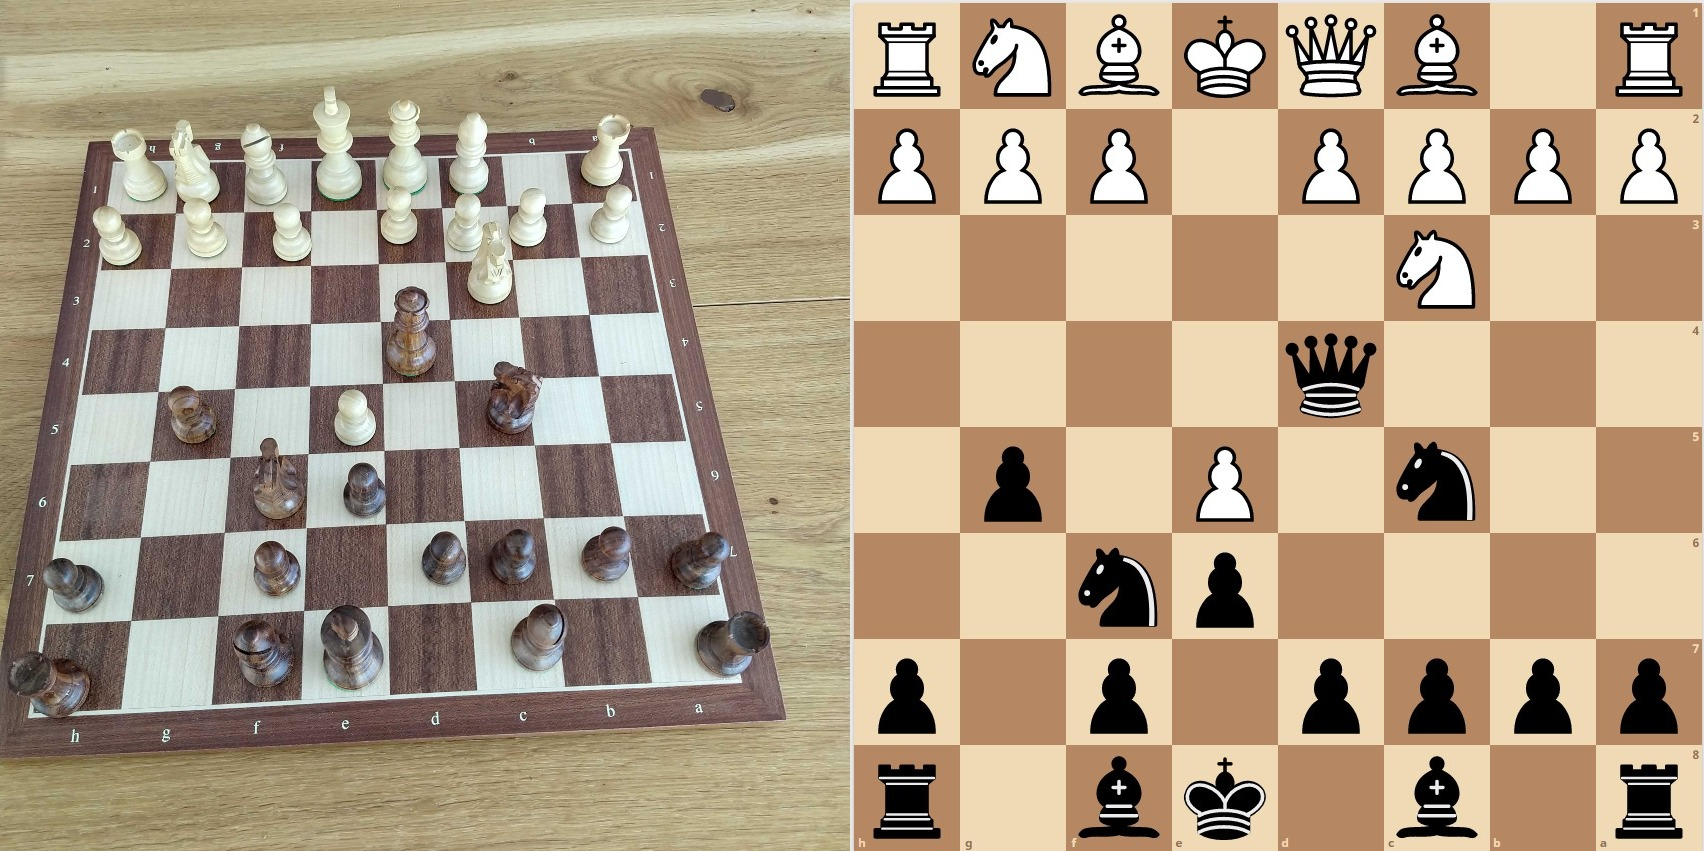
\includegraphics[width=1\textwidth]{../figures/introduction_img.jpg}
    \caption{Converting a physical chessboard into a digital one}
\end{figure}

\section{Board Detection and Rectification}

\subsection{Objective}
The primary goal of this part is to extract the 8$\times$8 chessboard from the raw video feed, then transform it into a top-down square image. This helps eliminate perspective distortion and background noise, such as the table, tripod or player movements, which could otherwise interfere with the analysis.

\subsection{Methodology}
The pipeline for board rectification is divided into three main processes:

\subsubsection*{A. Image Preprocessing - Edges Detection}
To extract the board structure, the frame is first converted to grayscale and smoothed using a \textbf{Gaussian Blur} with a $3\times3$ kernel to filter out high-frequency noise. We then apply a \textbf{Canny Edge Detector} to identify the grid boundaries. Finally, a \textbf{Morphological Closure} ($3\times3$ rect kernel) is performed to fill small gaps in the grid lines, ensuring a continuous contour regardless of lighting conditions.

\begin{figure}[h]
    \centering
    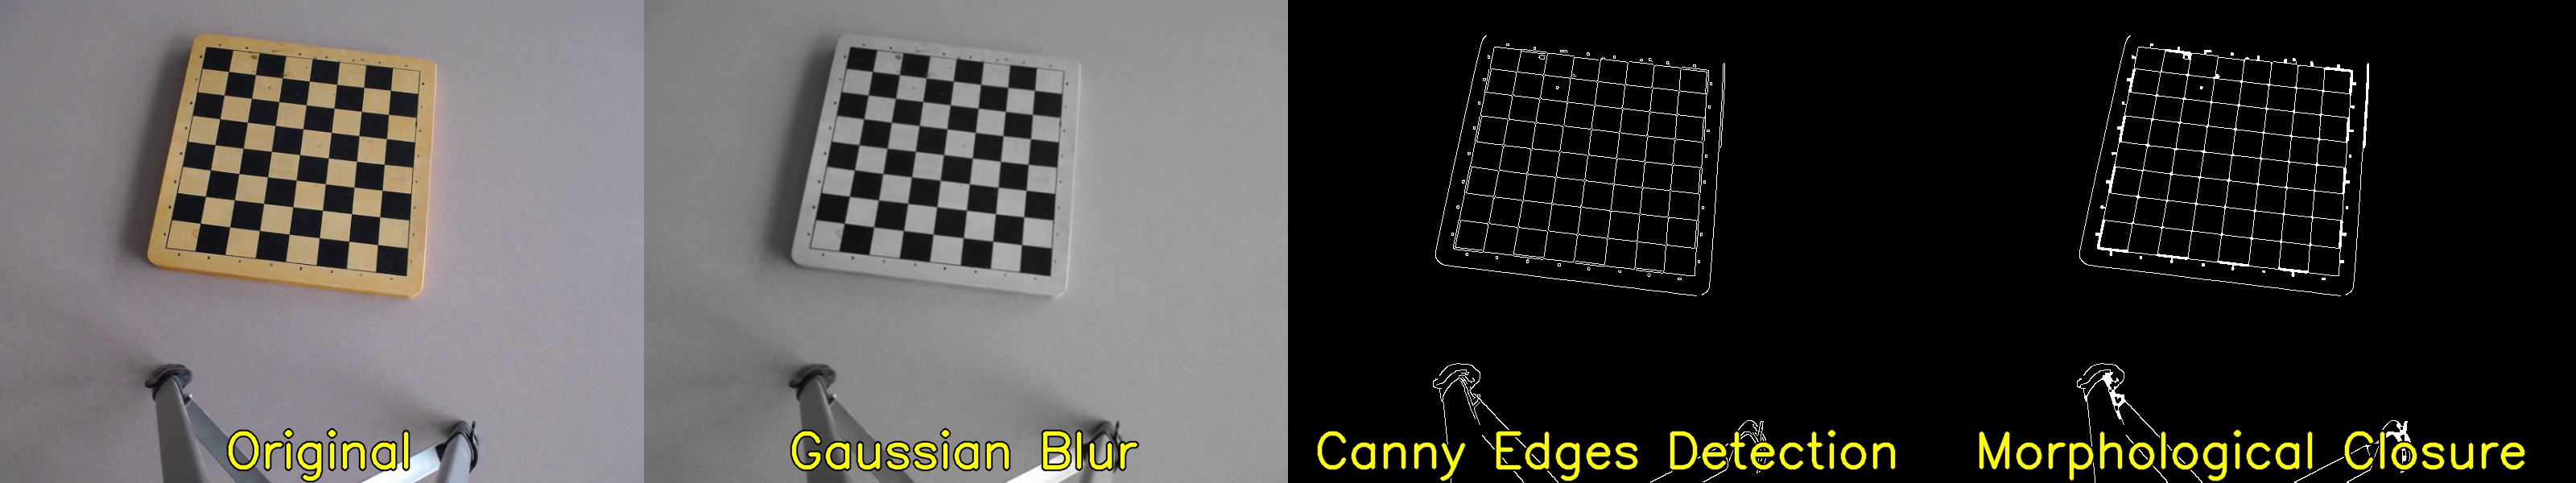
\includegraphics[width=1\textwidth]{../figures/preprocessing_workflow.jpg}
    \caption{Preprocessing Workflow: from the raw input to the closed-edge map}
\end{figure}

\subsubsection*{B. Corner Extraction}
The system identifies the chessboard by finding the largest external contour in the edge map, assuming the 8$\times$8 grid is the most suitable geometric feature. To extract the four specific corners from this contour, we use the following coordinate extremes:
\begin{itemize}
    \item \textbf{Top-Left}: Point with the minimum $(x + y)$ sum.
    \item \textbf{Bottom-Right}: Point with the maximum $(x + y)$ sum.
    \item \textbf{Top-Right}: Point with the minimum $(y - x)$ difference.
    \item \textbf{Bottom-Left}: Point with the maximum $(y - x)$ difference.
\end{itemize}

\subsubsection*{C. Perspective Transformation}
Once the corners are localized, a \textbf{Homography Matrix} is calculated using OpenCV's \texttt{getPerspectiveTransform}. This matrix maps the distorted coordinates to a perfect $400\times400$ pixel square. We then apply \texttt{warpPerspective} to generate the rectified ``top-down'' view ready for game transcription.

\subsection{Results and Discussion}

\begin{figure}[h]
    \centering
    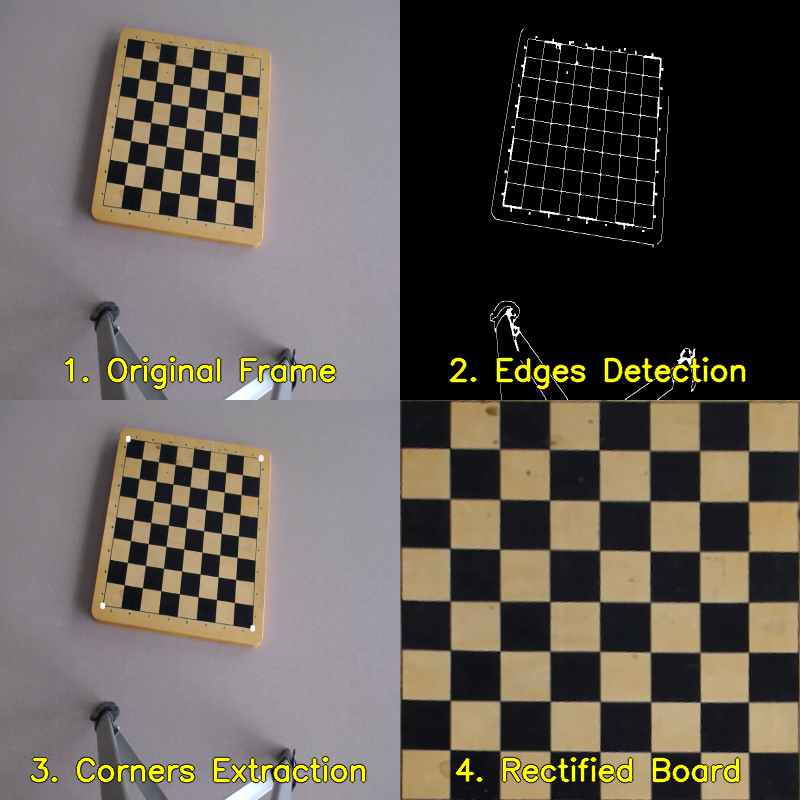
\includegraphics[width=0.6\textwidth]{../figures/part1_summary.png}
    \caption{Board Extraction Result}
\end{figure}

The implementation successfully generates a clean, standardized view of the board.
By extracting these corner coordinates from an empty-board video and storing them into \texttt{corners\_coordinates.json}, we have essentially \textbf{``locked''} the chessboard so that the system can remain stable thoughout the game.\\

While the rectified image simplifies determining cell occupancy, it is noted that the vertical shape of pieces may be distorted.
Consequently, while the rectified board is used for coordinate mapping, the \textit{original frame} may be referenced for piece identification to preserve visual features.



\end{CJK*}
\end{document}